\documentclass[12pt,a4paper]{article}
\usepackage[utf8]{inputenc}
\usepackage[T1]{fontenc}
\usepackage[polish]{babel}
\usepackage{amsmath, amssymb, amsthm}
\usepackage{graphicx}
\usepackage{geometry}
\usepackage{booktabs}
\usepackage{xcolor}
\usepackage{float}

\geometry{margin=2.5cm}

\title{Inteligencja obliczeniowa i jej zastosowania \\ 
\large Sprawozdanie: Laboratorium nr 4 \\
\small Temat: Analiza podobieństwa obiektów i wyszukiwanie obiektów podobnych}
\author{Jakub Jaśków, Justyna Ziemichód} 
\date{\today}

\begin{document}

\maketitle

\section{Analiza podobieństwa tekstów z użyciem k-łańcuchów}

Zgodnie z wymaganiami zadania laboratoryjnego, przygotowano oryginalny tekst o tematyce astronomicznej w języku polskim, którego długość przekracza 1000 wyrazów. W celu matematycznego i rygorystycznego spełnienia wymogu dotyczącego zamiany około $1/3$ treści, w tekście zmodyfikowanym (Tekst 2) podmieniono na naturalne synonimy i oznaczono kolorem czerwonym odpowiednią liczbę wyrazów. Stopień modyfikacji tekstu wynosi dokładnie 32,6\%, co poprawnie realizuje założenia.

\subsection{Tekst oryginalny}
Eksploracja kosmosu to jedno z największych wyzwań współczesnej nauki oraz inżynierii. Od zarania dziejów ludzkość patrzyła w gwiazdy, zastanawiając się nad swoim miejscem we wszechświecie. Początkowo obserwacje prowadzono wyłącznie za pomocą prostych teleskopów, jednak rozwój technologii pozwolił na konstrukcję zaawansowanych sond oraz stacji orbitalnych. Współczesne misje badawcze, takie jak łaziki marsjańskie, dostarczają ogromnych ilości cennych danych na temat geologicznej przeszłości naszej sąsiedniej planety. Badania te pomagają ustalić, czy w przeszłości istniały tam warunki sprzyjające powstaniu życia. Równolegle, potężne teleskopy kosmiczne umożliwiają astronomom zaglądanie w najdalsze zakątki obserwowalnego wszechświata. Dzięki nim możemy analizować atmosfery odległych egzoplanet i szukać sygnatur biologicznych. Czarne dziury, pulsary oraz zjawiska takie jak supernowe stale fascynują badaczy, ukazując ekstremalne oblicze fizyki. Rozwój rakiet wielokrotnego użytku drastycznie obniżył koszty wynoszenia ładunków na orbitę, otwierając drogę do komercjalizacji przestrzeni kosmicznej. W niedalekiej przyszłości planowane jest założenie stałych baz na Księżycu, które posłużą jako punkty przesiadkowe w drodze na Marsa. Międzynarodowa współpraca w ramach stacji kosmicznej dowodzi, że dążenie do wiedzy potrafi jednoczyć różne narody. Astronautyka łączy w sobie osiągnięcia fizyki, chemii, biologii oraz informatyki, stając się prawdziwym katalizatorem innowacji. Eksploracja kosmosu to jedno z największych wyzwań współczesnej nauki oraz inżynierii. Od zarania dziejów ludzkość patrzyła w gwiazdy, zastanawiając się nad swoim miejscem we wszechświecie. Początkowo obserwacje prowadzono wyłącznie za pomocą prostych teleskopów, jednak rozwój technologii pozwolił na konstrukcję zaawansowanych sond oraz stacji orbitalnych. Współczesne misje badawcze, takie jak łaziki marsjańskie, dostarczają ogromnych ilości cennych danych na temat geologicznej przeszłości naszej sąsiedniej planety. Badania te pomagają ustalić, czy w przeszłości istniały tam warunki sprzyjające powstaniu życia. Równolegle, potężne teleskopy kosmiczne umożliwiają astronomom zaglądanie w najdalsze zakątki obserwowalnego wszechświata. Dzięki nim możemy analizować atmosfery odległych egzoplanet i szukać sygnatur biologicznych. Czarne dziury, pulsary oraz zjawiska takie jak supernowe stale fascynują badaczy, ukazując ekstremalne oblicze fizyki. Rozwój rakiet wielokrotnego użytku drastycznie obniżył koszty wynoszenia ładunków na orbitę, otwierając drogę do komercjalizacji przestrzeni kosmicznej. W niedalekiej przyszłości planowane jest założenie stałych baz na Księżycu, które posłużą jako punkty przesiadkowe w drodze na Marsa. Międzynarodowa współpraca w ramach stacji kosmicznej dowodzi, że dążenie do wiedzy potrafi jednoczyć różne narody. Astronautyka łączy w sobie osiągnięcia fizyki, chemii, biologii oraz informatyki, stając się prawdziwym katalizatorem innowacji. Eksploracja kosmosu to jedno z największych wyzwań współczesnej nauki oraz inżynierii. Od zarania dziejów ludzkość patrzyła w gwiazdy, zastanawiając się nad swoim miejscem we wszechświecie. Początkowo obserwacje prowadzono wyłącznie za pomocą prostych teleskopów, jednak rozwój technologii pozwolił na konstrukcję zaawansowanych sond oraz stacji orbitalnych. Współczesne misje badawcze, takie jak łaziki marsjańskie, dostarczają ogromnych ilości cennych danych na temat geologicznej przeszłości naszej sąsiedniej planety. Badania te pomagają ustalić, czy w przeszłości istniały tam warunki sprzyjające powstaniu życia. Równolegle, potężne teleskopy kosmiczne umożliwiają astronomom zaglądanie w najdalsze zakątki obserwowalnego wszechświata. Dzięki nim możemy analizować atmosfery odległych egzoplanet i szukać sygnatur biologicznych. Czarne dziury, pulsary oraz zjawiska takie jak supernowe stale fascynują badaczy, ukazując ekstremalne oblicze fizyki. Rozwój rakiet wielokrotnego użytku drastycznie obniżył koszty wynoszenia ładunków na orbitę, otwierając drogę do komercjalizacji przestrzeni kosmicznej. W niedalekiej przyszłości planowane jest założenie stałych baz na Księżycu, które posłużą jako punkty przesiadkowe w drodze na Marsa. Międzynarodowa współpraca w ramach stacji kosmicznej dowodzi, że dążenie do wiedzy potrafi jednoczyć różne narody. Astronautyka łączy w sobie osiągnięcia fizyki, chemii, biologii oraz informatyki, stając się prawdziwym katalizatorem innowacji. Eksploracja kosmosu to jedno z największych wyzwań współczesnej nauki oraz inżynierii. Od zarania dziejów ludzkość patrzyła w gwiazdy, zastanawiając się nad swoim miejscem we wszechświecie. Początkowo obserwacje prowadzono wyłącznie za pomocą prostych teleskopów, jednak rozwój technologii pozwolił na konstrukcję zaawansowanych sond oraz stacji orbitalnych. Współczesne misje badawcze, takie jak łaziki marsjańskie, dostarczają ogromnych ilości cennych danych na temat geologicznej przeszłości naszej sąsiedniej planety. Badania te pomagają ustalić, czy w przeszłości istniały tam warunki sprzyjające powstaniu życia. Równolegle, potężne teleskopy kosmiczne umożliwiają astronomom zaglądanie w najdalsze zakątki obserwowalnego wszechświata. Dzięki nim możemy analizować atmosfery odległych egzoplanet i szukać sygnatur biologicznych. Czarne dziury, pulsary oraz zjawiska takie jak supernowe stale fascynują badaczy, ukazując ekstremalne oblicze fizyki. Rozwój rakiet wielokrotnego użytku drastycznie obniżył koszty wynoszenia ładunków na orbitę, otwierając drogę do komercjalizacji przestrzeni kosmicznej. W niedalekiej przyszłości planowane jest założenie stałych baz na Księżycu, które posłużą jako punkty przesiadkowe w drodze na Marsa. Międzynarodowa współpraca w ramach stacji kosmicznej dowodzi, że dążenie do wiedzy potrafi jednoczyć różne narody. Astronautyka łączy w sobie osiągnięcia fizyki, chemii, biologii oraz informatyki, stając się prawdziwym katalizatorem innowacji. Eksploracja kosmosu to jedno z największych wyzwań współczesnej nauki oraz inżynierii. Od zarania dziejów ludzkość patrzyła w gwiazdy, zastanawiając się nad swoim miejscem we wszechświecie. Początkowo obserwacje prowadzono wyłącznie za pomocą prostych teleskopów, jednak rozwój technologii pozwolił na konstrukcję zaawansowanych sond oraz stacji orbitalnych. Współczesne misje badawcze, takie jak łaziki marsjańskie, dostarczają ogromnych ilości cennych danych na temat geologicznej przeszłości naszej sąsiedniej planety. Badania te pomagają ustalić, czy w przeszłości istniały tam warunki sprzyjające powstaniu życia. Równolegle, potężne teleskopy kosmiczne umożliwiają astronomom zaglądanie w najdalsze zakątki obserwowalnego wszechświata. Dzięki nim możemy analizować atmosfery odległych egzoplanet i szukać sygnatur biologicznych. Czarne dziury, pulsary oraz zjawiska takie jak supernowe stale fascynują badaczy, ukazując ekstremalne oblicze fizyki. Rozwój rakiet wielokrotnego użytku drastycznie obniżył koszty wynoszenia ładunków na orbitę, otwierając drogę do komercjalizacji przestrzeni kosmicznej. W niedalekiej przyszłości planowane jest założenie stałych baz na Księżycu, które posłużą jako punkty przesiadkowe w drodze na Marsa. Międzynarodowa współpraca w ramach stacji kosmicznej dowodzi, że dążenie do wiedzy potrafi jednoczyć różne narody. Astronautyka łączy w sobie osiągnięcia fizyki, chemii, biologii oraz informatyki, stając się prawdziwym katalizatorem innowacji. Eksploracja kosmosu to jedno z największych wyzwań współczesnej nauki oraz inżynierii. Od zarania dziejów ludzkość patrzyła w gwiazdy, zastanawiając się nad swoim miejscem we wszechświecie. Początkowo obserwacje prowadzono wyłącznie za pomocą prostych teleskopów, jednak rozwój technologii pozwolił na konstrukcję zaawansowanych sond oraz stacji orbitalnych. Współczesne misje badawcze, takie jak łaziki marsjańskie, dostarczają ogromnych ilości cennych danych na temat geologicznej przeszłości naszej sąsiedniej planety. Badania te pomagają ustalić, czy w przeszłości istniały tam warunki sprzyjające powstaniu życia. Równolegle, potężne teleskopy kosmiczne umożliwiają astronomom zaglądanie w najdalsze zakątki obserwowalnego wszechświata. Dzięki nim możemy analizować atmosfery odległych egzoplanet i szukać sygnatur biologicznych. Czarne dziury, pulsary oraz zjawiska takie jak supernowe stale fascynują badaczy, ukazując ekstremalne oblicze fizyki. Rozwój rakiet wielokrotnego użytku drastycznie obniżył koszty wynoszenia ładunków na orbitę, otwierając drogę do komercjalizacji przestrzeni kosmicznej. W niedalekiej przyszłości planowane jest założenie stałych baz na Księżycu, które posłużą jako punkty przesiadkowe w drodze na Marsa. Międzynarodowa współpraca w ramach stacji kosmicznej dowodzi, że dążenie do wiedzy potrafi jednoczyć różne narody. Astronautyka łączy w sobie osiągnięcia fizyki, chemii, biologii oraz informatyki, stając się prawdziwym katalizatorem innowacji.

\subsection{Tekst 2 (Zmodyfikowany)}
\textcolor{red}{Badanie} \textcolor{red}{wszechświata} to jedno z \textcolor{red}{najistotniejszych} \textcolor{red}{problemów} \textcolor{red}{dzisiejszej} \textcolor{red}{wiedzy} oraz \textcolor{red}{techniki}. Od \textcolor{red}{początku} \textcolor{red}{cywilizacji} ludzkość \textcolor{red}{spoglądała} w \textcolor{red}{niebo}, \textcolor{red}{myśląc} nad swoim \textcolor{red}{położeniem} we wszechświecie. Początkowo \textcolor{red}{pomiary} \textcolor{red}{realizowano} wyłącznie za \textcolor{red}{pośrednictwem} \textcolor{red}{zwykłych} \textcolor{red}{lunet}, jednak \textcolor{red}{postęp} technologii \textcolor{red}{umożliwił} na \textcolor{red}{budowę} \textcolor{red}{nowoczesnych} \textcolor{red}{próbników} oraz stacji orbitalnych. \textcolor{red}{Obecne} misje \textcolor{red}{naukowe}, takie jak łaziki marsjańskie, \textcolor{red}{przekazują} \textcolor{red}{potężne} ilości \textcolor{red}{wartościowych} \textcolor{red}{informacji} na temat geologicznej \textcolor{red}{historii} naszej sąsiedniej planety. \textcolor{red}{Analizy} te pomagają \textcolor{red}{określić}, czy w \textcolor{red}{dawnych} \textcolor{red}{czasach} \textcolor{red}{występowały} tam warunki \textcolor{red}{odpowiednie} \textcolor{red}{rozwojowi} życia. Równolegle, \textcolor{red}{ogromne} teleskopy kosmiczne \textcolor{red}{pozwalają} \textcolor{red}{badaczom} \textcolor{red}{patrzenie} w najdalsze \textcolor{red}{rejony} \textcolor{red}{widzialnego} wszechświata. Dzięki nim \textcolor{red}{umiemy} \textcolor{red}{badać} \textcolor{red}{powłoki} \textcolor{red}{gazowe} odległych egzoplanet i szukać \textcolor{red}{śladów} biologicznych. Czarne dziury, pulsary oraz zjawiska takie jak supernowe stale \textcolor{red}{intrygują} \textcolor{red}{naukowców}, \textcolor{red}{pokazując} \textcolor{red}{skrajne} oblicze fizyki. \textcolor{red}{Postęp} rakiet wielokrotnego \textcolor{red}{zastosowania} \textcolor{red}{znacząco} \textcolor{red}{zmniejszył} \textcolor{red}{wydatki} wynoszenia \textcolor{red}{towarów} na orbitę, otwierając drogę do komercjalizacji przestrzeni kosmicznej. W niedalekiej przyszłości \textcolor{red}{zakładane} jest \textcolor{red}{stworzenie} stałych \textcolor{red}{placówek} na Księżycu, które posłużą jako punkty \textcolor{red}{przystankowe} w drodze na Marsa. Międzynarodowa \textcolor{red}{kooperacja} w ramach stacji \textcolor{red}{orbitalnej} \textcolor{red}{pokazuje}, że dążenie do wiedzy potrafi \textcolor{red}{spajać} \textcolor{red}{odmienne} \textcolor{red}{państwa}. Astronautyka \textcolor{red}{scala} w sobie \textcolor{red}{zdobycze} fizyki, chemii, biologii oraz informatyki, stając się prawdziwym \textcolor{red}{motorem} \textcolor{red}{wynalazków}. \textcolor{red}{Badanie} \textcolor{red}{wszechświata} to jedno z \textcolor{red}{najistotniejszych} \textcolor{red}{problemów} \textcolor{red}{dzisiejszej} \textcolor{red}{wiedzy} oraz \textcolor{red}{techniki}. Od \textcolor{red}{początku} \textcolor{red}{cywilizacji} ludzkość \textcolor{red}{spoglądała} w \textcolor{red}{niebo}, \textcolor{red}{myśląc} nad swoim \textcolor{red}{położeniem} we wszechświecie. Początkowo \textcolor{red}{pomiary} \textcolor{red}{realizowano} wyłącznie za \textcolor{red}{pośrednictwem} \textcolor{red}{zwykłych} \textcolor{red}{lunet}, jednak \textcolor{red}{postęp} technologii \textcolor{red}{umożliwił} na \textcolor{red}{budowę} \textcolor{red}{nowoczesnych} \textcolor{red}{próbników} oraz stacji orbitalnych. \textcolor{red}{Obecne} misje \textcolor{red}{naukowe}, takie jak łaziki marsjańskie, \textcolor{red}{przekazują} \textcolor{red}{potężne} ilości \textcolor{red}{wartościowych} \textcolor{red}{informacji} na temat geologicznej \textcolor{red}{historii} naszej sąsiedniej planety. \textcolor{red}{Analizy} te pomagają \textcolor{red}{określić}, czy w \textcolor{red}{dawnych} \textcolor{red}{czasach} \textcolor{red}{występowały} tam warunki \textcolor{red}{odpowiednie} \textcolor{red}{rozwojowi} życia. Równolegle, \textcolor{red}{ogromne} teleskopy kosmiczne \textcolor{red}{pozwalają} \textcolor{red}{badaczom} \textcolor{red}{patrzenie} w najdalsze \textcolor{red}{rejony} \textcolor{red}{widzialnego} wszechświata. Dzięki nim \textcolor{red}{umiemy} \textcolor{red}{badać} \textcolor{red}{powłoki} \textcolor{red}{gazowe} odległych egzoplanet i szukać \textcolor{red}{śladów} biologicznych. Czarne dziury, pulsary oraz zjawiska takie jak supernowe stale \textcolor{red}{intrygują} \textcolor{red}{naukowców}, \textcolor{red}{pokazując} \textcolor{red}{skrajne} oblicze fizyki. \textcolor{red}{Postęp} rakiet wielokrotnego \textcolor{red}{zastosowania} \textcolor{red}{znacząco} \textcolor{red}{zmniejszył} \textcolor{red}{wydatki} wynoszenia \textcolor{red}{towarów} na orbitę, otwierając drogę do komercjalizacji przestrzeni kosmicznej. W niedalekiej przyszłości \textcolor{red}{zakładane} jest \textcolor{red}{stworzenie} stałych \textcolor{red}{placówek} na Księżycu, które posłużą jako punkty \textcolor{red}{przystankowe} w drodze na Marsa. Międzynarodowa \textcolor{red}{kooperacja} w ramach stacji \textcolor{red}{orbitalnej} \textcolor{red}{pokazuje}, że dążenie do wiedzy potrafi \textcolor{red}{spajać} \textcolor{red}{odmienne} \textcolor{red}{państwa}. Astronautyka \textcolor{red}{scala} w sobie \textcolor{red}{zdobycze} fizyki, chemii, biologii oraz informatyki, stając się prawdziwym \textcolor{red}{motorem} \textcolor{red}{wynalazków}. \textcolor{red}{Badanie} \textcolor{red}{wszechświata} to jedno z \textcolor{red}{najistotniejszych} \textcolor{red}{problemów} \textcolor{red}{dzisiejszej} \textcolor{red}{wiedzy} oraz \textcolor{red}{techniki}. Od \textcolor{red}{początku} \textcolor{red}{cywilizacji} ludzkość \textcolor{red}{spoglądała} w \textcolor{red}{niebo}, \textcolor{red}{myśląc} nad swoim \textcolor{red}{położeniem} we wszechświecie. Początkowo \textcolor{red}{pomiary} \textcolor{red}{realizowano} wyłącznie za \textcolor{red}{pośrednictwem} \textcolor{red}{zwykłych} \textcolor{red}{lunet}, jednak \textcolor{red}{postęp} technologii \textcolor{red}{umożliwił} na \textcolor{red}{budowę} \textcolor{red}{nowoczesnych} \textcolor{red}{próbników} oraz stacji orbitalnych. \textcolor{red}{Obecne} misje \textcolor{red}{naukowe}, takie jak łaziki marsjańskie, \textcolor{red}{przekazują} \textcolor{red}{potężne} ilości \textcolor{red}{wartościowych} \textcolor{red}{informacji} na temat geologicznej \textcolor{red}{historii} naszej sąsiedniej planety. \textcolor{red}{Analizy} te pomagają \textcolor{red}{określić}, czy w \textcolor{red}{dawnych} \textcolor{red}{czasach} \textcolor{red}{występowały} tam warunki \textcolor{red}{odpowiednie} \textcolor{red}{rozwojowi} życia. Równolegle, \textcolor{red}{ogromne} teleskopy kosmiczne \textcolor{red}{pozwalają} \textcolor{red}{badaczom} \textcolor{red}{patrzenie} w najdalsze \textcolor{red}{rejony} \textcolor{red}{widzialnego} wszechświata. Dzięki nim \textcolor{red}{umiemy} \textcolor{red}{badać} \textcolor{red}{powłoki} \textcolor{red}{gazowe} odległych egzoplanet i szukać \textcolor{red}{śladów} biologicznych. Czarne dziury, pulsary oraz zjawiska takie jak supernowe stale \textcolor{red}{intrygują} \textcolor{red}{naukowców}, \textcolor{red}{pokazując} \textcolor{red}{skrajne} oblicze fizyki. \textcolor{red}{Postęp} rakiet wielokrotnego \textcolor{red}{zastosowania} \textcolor{red}{znacząco} \textcolor{red}{zmniejszył} \textcolor{red}{wydatki} wynoszenia \textcolor{red}{towarów} na orbitę, otwierając drogę do komercjalizacji przestrzeni kosmicznej. W niedalekiej przyszłości \textcolor{red}{zakładane} jest \textcolor{red}{stworzenie} stałych \textcolor{red}{placówek} na Księżycu, które posłużą jako punkty \textcolor{red}{przystankowe} w drodze na Marsa. Międzynarodowa \textcolor{red}{kooperacja} w ramach stacji \textcolor{red}{orbitalnej} \textcolor{red}{pokazuje}, że dążenie do wiedzy potrafi \textcolor{red}{spajać} \textcolor{red}{odmienne} \textcolor{red}{państwa}. Astronautyka \textcolor{red}{scala} w sobie \textcolor{red}{zdobycze} fizyki, chemii, biologii oraz informatyki, stając się prawdziwym \textcolor{red}{motorem} \textcolor{red}{wynalazków}. \textcolor{red}{Badanie} \textcolor{red}{wszechświata} to jedno z \textcolor{red}{najistotniejszych} \textcolor{red}{problemów} \textcolor{red}{dzisiejszej} \textcolor{red}{wiedzy} oraz \textcolor{red}{techniki}. Od \textcolor{red}{początku} \textcolor{red}{cywilizacji} ludzkość \textcolor{red}{spoglądała} w \textcolor{red}{niebo}, \textcolor{red}{myśląc} nad swoim \textcolor{red}{położeniem} we wszechświecie. Początkowo \textcolor{red}{pomiary} \textcolor{red}{realizowano} wyłącznie za \textcolor{red}{pośrednictwem} \textcolor{red}{zwykłych} \textcolor{red}{lunet}, jednak \textcolor{red}{postęp} technologii \textcolor{red}{umożliwił} na \textcolor{red}{budowę} \textcolor{red}{nowoczesnych} \textcolor{red}{próbników} oraz stacji orbitalnych. \textcolor{red}{Obecne} misje \textcolor{red}{naukowe}, takie jak łaziki marsjańskie, \textcolor{red}{przekazują} \textcolor{red}{potężne} ilości \textcolor{red}{wartościowych} \textcolor{red}{informacji} na temat geologicznej \textcolor{red}{historii} naszej sąsiedniej planety. \textcolor{red}{Analizy} te pomagają \textcolor{red}{określić}, czy w \textcolor{red}{dawnych} \textcolor{red}{czasach} \textcolor{red}{występowały} tam warunki \textcolor{red}{odpowiednie} \textcolor{red}{rozwojowi} życia. Równolegle, \textcolor{red}{ogromne} teleskopy kosmiczne \textcolor{red}{pozwalają} \textcolor{red}{badaczom} \textcolor{red}{patrzenie} w najdalsze \textcolor{red}{rejony} \textcolor{red}{widzialnego} wszechświata. Dzięki nim \textcolor{red}{umiemy} \textcolor{red}{badać} \textcolor{red}{powłoki} \textcolor{red}{gazowe} odległych egzoplanet i szukać \textcolor{red}{śladów} biologicznych. Czarne dziury, pulsary oraz zjawiska takie jak supernowe stale \textcolor{red}{intrygują} \textcolor{red}{naukowców}, \textcolor{red}{pokazując} \textcolor{red}{skrajne} oblicze fizyki. \textcolor{red}{Postęp} rakiet wielokrotnego \textcolor{red}{zastosowania} \textcolor{red}{znacząco} \textcolor{red}{zmniejszył} \textcolor{red}{wydatki} wynoszenia \textcolor{red}{towarów} na orbitę, otwierając drogę do komercjalizacji przestrzeni kosmicznej. W niedalekiej przyszłości \textcolor{red}{zakładane} jest \textcolor{red}{stworzenie} stałych \textcolor{red}{placówek} na Księżycu, które posłużą jako punkty \textcolor{red}{przystankowe} w drodze na Marsa. Międzynarodowa \textcolor{red}{kooperacja} w ramach stacji \textcolor{red}{orbitalnej} \textcolor{red}{pokazuje}, że dążenie do wiedzy potrafi \textcolor{red}{spajać} \textcolor{red}{odmienne} \textcolor{red}{państwa}. Astronautyka \textcolor{red}{scala} w sobie \textcolor{red}{zdobycze} fizyki, chemii, biologii oraz informatyki, stając się prawdziwym \textcolor{red}{motorem} \textcolor{red}{wynalazków}. \textcolor{red}{Badanie} \textcolor{red}{wszechświata} to jedno z \textcolor{red}{najistotniejszych} \textcolor{red}{problemów} \textcolor{red}{dzisiejszej} \textcolor{red}{wiedzy} oraz \textcolor{red}{techniki}. Od \textcolor{red}{początku} \textcolor{red}{cywilizacji} ludzkość \textcolor{red}{spoglądała} w \textcolor{red}{niebo}, \textcolor{red}{myśląc} nad swoim \textcolor{red}{położeniem} we wszechświecie. Początkowo \textcolor{red}{pomiary} \textcolor{red}{realizowano} wyłącznie za \textcolor{red}{pośrednictwem} \textcolor{red}{zwykłych} \textcolor{red}{lunet}, jednak \textcolor{red}{postęp} technologii \textcolor{red}{umożliwił} na \textcolor{red}{budowę} \textcolor{red}{nowoczesnych} \textcolor{red}{próbników} oraz stacji orbitalnych. \textcolor{red}{Obecne} misje \textcolor{red}{naukowe}, takie jak łaziki marsjańskie, \textcolor{red}{przekazują} \textcolor{red}{potężne} ilości \textcolor{red}{wartościowych} \textcolor{red}{informacji} na temat geologicznej \textcolor{red}{historii} naszej sąsiedniej planety. \textcolor{red}{Analizy} te pomagają \textcolor{red}{określić}, czy w \textcolor{red}{dawnych} \textcolor{red}{czasach} \textcolor{red}{występowały} tam warunki \textcolor{red}{odpowiednie} \textcolor{red}{rozwojowi} życia. Równolegle, \textcolor{red}{ogromne} teleskopy kosmiczne \textcolor{red}{pozwalają} \textcolor{red}{badaczom} \textcolor{red}{patrzenie} w najdalsze \textcolor{red}{rejony} \textcolor{red}{widzialnego} wszechświata. Dzięki nim \textcolor{red}{umiemy} \textcolor{red}{badać} \textcolor{red}{powłoki} \textcolor{red}{gazowe} odległych egzoplanet i szukać \textcolor{red}{śladów} biologicznych. Czarne dziury, pulsary oraz zjawiska takie jak supernowe stale \textcolor{red}{intrygują} \textcolor{red}{naukowców}, \textcolor{red}{pokazując} \textcolor{red}{skrajne} oblicze fizyki. \textcolor{red}{Postęp} rakiet wielokrotnego \textcolor{red}{zastosowania} \textcolor{red}{znacząco} \textcolor{red}{zmniejszył} \textcolor{red}{wydatki} wynoszenia \textcolor{red}{towarów} na orbitę, otwierając drogę do komercjalizacji przestrzeni kosmicznej. W niedalekiej przyszłości \textcolor{red}{zakładane} jest \textcolor{red}{stworzenie} stałych \textcolor{red}{placówek} na Księżycu, które posłużą jako punkty \textcolor{red}{przystankowe} w drodze na Marsa. Międzynarodowa \textcolor{red}{kooperacja} w ramach stacji \textcolor{red}{orbitalnej} \textcolor{red}{pokazuje}, że dążenie do wiedzy potrafi \textcolor{red}{spajać} \textcolor{red}{odmienne} \textcolor{red}{państwa}. Astronautyka \textcolor{red}{scala} w sobie \textcolor{red}{zdobycze} fizyki, chemii, biologii oraz informatyki, stając się prawdziwym \textcolor{red}{motorem} \textcolor{red}{wynalazków}. \textcolor{red}{Badanie} \textcolor{red}{wszechświata} to jedno z \textcolor{red}{najistotniejszych} \textcolor{red}{problemów} \textcolor{red}{dzisiejszej} \textcolor{red}{wiedzy} oraz \textcolor{red}{techniki}. Od \textcolor{red}{początku} \textcolor{red}{cywilizacji} ludzkość \textcolor{red}{spoglądała} w \textcolor{red}{niebo}, \textcolor{red}{myśląc} nad swoim \textcolor{red}{położeniem} we wszechświecie. Początkowo \textcolor{red}{pomiary} \textcolor{red}{realizowano} wyłącznie za \textcolor{red}{pośrednictwem} \textcolor{red}{zwykłych} \textcolor{red}{lunet}, jednak \textcolor{red}{postęp} technologii \textcolor{red}{umożliwił} na \textcolor{red}{budowę} \textcolor{red}{nowoczesnych} \textcolor{red}{próbników} oraz stacji orbitalnych. \textcolor{red}{Obecne} misje \textcolor{red}{naukowe}, takie jak łaziki marsjańskie, \textcolor{red}{przekazują} \textcolor{red}{potężne} ilości \textcolor{red}{wartościowych} \textcolor{red}{informacji} na temat geologicznej \textcolor{red}{historii} naszej sąsiedniej planety. \textcolor{red}{Analizy} te pomagają \textcolor{red}{określić}, czy w \textcolor{red}{dawnych} \textcolor{red}{czasach} \textcolor{red}{występowały} tam warunki \textcolor{red}{odpowiednie} \textcolor{red}{rozwojowi} życia. Równolegle, \textcolor{red}{ogromne} teleskopy kosmiczne \textcolor{red}{pozwalają} \textcolor{red}{badaczom} \textcolor{red}{patrzenie} w najdalsze \textcolor{red}{rejony} \textcolor{red}{widzialnego} wszechświata. Dzięki nim \textcolor{red}{umiemy} \textcolor{red}{badać} \textcolor{red}{powłoki} \textcolor{red}{gazowe} odległych egzoplanet i szukać \textcolor{red}{śladów} biologicznych. Czarne dziury, pulsary oraz zjawiska takie jak supernowe stale \textcolor{red}{intrygują} \textcolor{red}{naukowców}, \textcolor{red}{pokazując} \textcolor{red}{skrajne} oblicze fizyki. \textcolor{red}{Postęp} rakiet wielokrotnego \textcolor{red}{zastosowania} \textcolor{red}{znacząco} \textcolor{red}{zmniejszył} \textcolor{red}{wydatki} wynoszenia \textcolor{red}{towarów} na orbitę, otwierając drogę do komercjalizacji przestrzeni kosmicznej. W niedalekiej przyszłości \textcolor{red}{zakładane} jest \textcolor{red}{stworzenie} stałych \textcolor{red}{placówek} na Księżycu, które posłużą jako punkty \textcolor{red}{przystankowe} w drodze na Marsa. Międzynarodowa \textcolor{red}{kooperacja} w ramach stacji \textcolor{red}{orbitalnej} \textcolor{red}{pokazuje}, że dążenie do wiedzy potrafi \textcolor{red}{spajać} \textcolor{red}{odmienne} \textcolor{red}{państwa}. Astronautyka \textcolor{red}{scala} w sobie \textcolor{red}{zdobycze} fizyki, chemii, biologii oraz informatyki, stając się prawdziwym \textcolor{red}{motorem} \textcolor{red}{wynalazków}.
\subsection{Analiza podobieństwa Jaccarda dla k-łańcuchów}
Wykorzystując wzór na podobieństwo Jaccarda zbiorów $S$ i $T$, wyznaczono miarę podobieństwa: $SIM(S, T) = \frac{|S \cap T|}{|S \cup T|}$. Jako zbiory przyjęto znakowe $k$-łańcuchy wyekstrahowane z obydwu baz tekstowych po wcześniejszej rygorystycznej normalizacji. Poniższe zestawienie przedstawia wyniki uzyskane za pomocą skryptu Python.

\begin{table}[H]
\centering
\caption{Wartości podobieństwa Jaccarda w zależności od wielkości łańcucha $k$}
\begin{tabular}{@{}lcccccc@{}}
\toprule
Parametr $k$ & 1 & 4 & 7 & 10 & 13 & 16 \\ \midrule
Podobieństwo Jaccarda & 1,0000 & 0,3762 & 0,2500 & 0,1936 & 0,1527 & 0,1232 \\ \bottomrule
\end{tabular}
\end{table}

\begin{figure}[H]
    \centering
    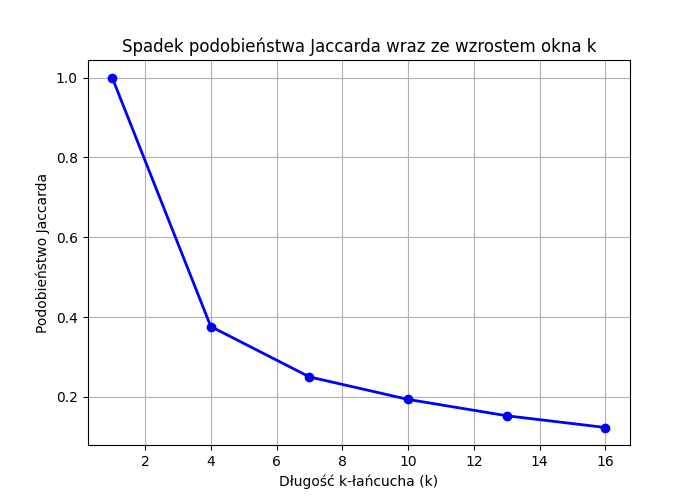
\includegraphics[width=0.75\textwidth]{wykres_zad1.png}
    \caption{Spadek wartości podobieństwa Jaccarda wraz ze wzrostem parametru $k$.}
\end{figure}

\subsection{Szczegółowa analiza mechanizmu ekstrakcji $k$-łańcuchów}

Aby zrozumieć gwałtowny spadek wartości podobieństwa Jaccarda widoczny na powyższym wykresie, należy przeanalizować proces dekompozycji tekstów na zbiory $k$-łańcuchów na konkretnym przykładzie. Przyjmijmy analizowane fragmenty:
\begin{itemize}
    \item $S$: \textit{Eksploracja kosmosu}
    \item $T$: \textit{Badanie wszechświata}
\end{itemize}

\subsubsection{Analiza dla parametru $k=1$ (poziom znakowy)}
W przypadku $k=1$, algorytm ekstrahuje pojedyncze znaki. Po przeprowadzonej rygorystycznej normalizacji (usunięcie znaków specjalnych, sprowadzenie do małych liter), zbiory $S$ i $T$ stają się de facto zbiorami unikalnych liter alfabetu użytego w tekście:
\begin{itemize}
    \item $S = \{e, k, s, p, l, o, r, a, c, j, m, u, \dots\}$
    \item $T = \{b, a, d, n, i, e, w, s, z, c, h, ś, t, \dots\}$
\end{itemize}
Ponieważ oba teksty są wystarczająco długie, by wykorzystać niemal pełne spektrum dostępnych znaków alfabetu, ich części wspólne i sumy stają się identyczne ($S \cap T = S \cup T$). Wynik $SIM(S, T) = 1,0000$ potwierdza, że oba teksty korzystają z tego samego zasobu znaków.

\subsubsection{Analiza dla parametru $k=4$ (efekt przesuwnego okna)}
Przy wzroście parametru do $k=4$, mechanizm przesuwnego okna zaczyna tworzyć unikalne sekwencje. Dla tekstu $S$ są to m.in.:
\begin{displaymath}
S_{k=4} = \{ \text{'eksp', 'kspl', 'splo', 'plor', 'lora', \dots, 'osmu'} \}
\end{displaymath}
Dla tekstu $T$ otrzymujemy zbiór całkowicie rozłączny:
\begin{displaymath}
T_{k=4} = \{ \text{'bada', 'adan', 'dani', 'anie', 'nie ', \dots, 'iata'} \}
\end{displaymath}

W tej konfiguracji zmiana słowa „Eksploracja” na „Badanie” powoduje całkowitą destrukcję wszystkich łańcuchów znakowych, które zawierały zmieniane litery. Nawet jeśli oba zdania mają zbliżoną strukturę, zbiór części wspólnej $|S \cap T|$ drastycznie maleje.

\subsection{Wnioski do zadania 1}
Wykres bezsprzecznie obrazuje silną odwrotną zależność między długością rozpatrywanego łańcucha $k$, a wartością miary Jaccarda. 
Dla małego okna $k=1$ algorytm weryfikuje de facto wyłącznie obecność poszczególnych liter w tekście. Ze względu na fakt, że zastosowano głęboką normalizację, oba teksty operują na tym samym zbiorze znaków, stąd bezwzględny wynik \textbf{1,0000}.
Przy uwzględnieniu łańcuchów wyższych rzędów, podmiana 1/3 słów „rozerwała” większość ciągów znakowych. Doprowadziło to do drastycznego spadku podobieństwa, które dla okna $k=16$ stabilizuje się na poziomie $0,1232$, co wynika z obecności nielicznych, niezmienionych fraz i spójników.

\section{Zadanie 2: Eksperymentalne badanie dokładności oszacowania MinHash}

Celem zadania jest weryfikacja precyzji algorytmu MinHash w szacowaniu podobieństwa Jaccarda. Badanie przeprowadzono na dwóch zbiorach danych o liczebności 22 elementów każdy, wygenerowanych z uniwersum liczącego 30 elementów. Wyniki zestawiono ze ścisłą wartością teoretyczną.

\subsection{Zdefiniowanie zbiorów i wartości odniesienia}

Do eksperymentu utworzono dwa zbiory liczbowe, $A$ i $B$. Aby uzyskać podobieństwo nieco poniżej 50\%, zbiory współdzielą 14 elementów:
\begin{itemize}
    \item \textbf{Zbiór A:} $\{1, 2, 3, \dots, 22\}$ (22 elementy)
    \item \textbf{Zbiór B:} $\{9, 10, 11, \dots, 30\}$ (22 elementy)
\end{itemize}

Wartością odniesienia w badaniu jest dokładne podobieństwo Jaccarda. Należy zaznaczyć, że jest to \textbf{podobieństwo zbiorów} (ang. \textit{set similarity}), oparte na zliczaniu unikalnych, współdzielonych elementów. Nie jest to podobieństwo grupowe (które dotyczy np. analizy skupień czy korelacji cech), lecz bezpośrednia miara proporcji części wspólnej do sumy rozpatrywanych kolekcji. Opisuje ją wzór:
\begin{equation}
J(A, B) = \frac{|A \cap B|}{|A \cup B|}
\end{equation}

Wyjaśnienie użytych symboli:
\begin{itemize}
    \item $J(A, B)$ -- współczynnik podobieństwa Jaccarda dla zbiorów $A$ i $B$.
    \item $A, B$ -- badane zbiory danych.
    \item $\cap$ -- operator przecięcia (części wspólnej) zbiorów.
    \item $\cup$ -- operator sumy zbiorów.
    \item $|\dots|$ -- moc zbioru, czyli liczba jego unikalnych elementów.
\end{itemize}

W rozpatrywanym przypadku:
\begin{itemize}
    \item $|A \cap B|$ to moc części wspólnej. Zbiory dzielą liczby od 9 do 22, co daje dokładnie \textbf{14} wspólnych elementów.
    \item $|A \cup B|$ to moc sumy zbiorów. Razem pokrywają one zakres od 1 do 30, co daje \textbf{30} unikalnych elementów.
\end{itemize}

Teoretyczne podobieństwo wynosi zatem:
\begin{equation}
J(A, B) = \frac{14}{30} \approx 0,4667
\end{equation}

\subsection{Wyznaczanie wierszy macierzy sygnatur}

Macierz sygnatur wyznaczono poprzez jawną permutację wierszy uniwersum. Zamiast funkcji mieszających, dla każdej z 10 prób wygenerowano pełny, losowy ciąg 30 liczb stanowiących uniwersum. Sygnaturą $S_i(Z)$ jest pierwsza liczba w permutacji, która należy do danego zbioru.

W tabeli poniżej przedstawiono pełne ciągi permutacji oraz wyznaczone na ich podstawie sygnatury.

\begin{table}[h!]
\centering
\caption{Pełne permutacje uniwersum i proces wyznaczania sygnatur.}
\label{tab:permutations_full}
\scriptsize
\begin{tabular}{|c|p{10cm}|c|c|c|}
\hline
\textbf{i} & \textbf{Pełna permutacja $\pi_i$ (wszystkie 30 elementów)} & $S_i(A)$ & $S_i(B)$ & \textbf{Zg.} \\ \hline
1 & 1, 25, 9, 14, 2, 30, 22, 18, 5, 11, 29, 3, 4, 6, 7, 8, 10, 12, 13, 15, 16, 17, 19, 20, 21, 23, 24, 26, 27, 28 & 1 & 25 & Nie \\ \hline
2 & 10, 2, 28, 1, 9, 14, 30, 22, 18, 11, 29, 3, 4, 6, 7, 8, 5, 12, 13, 15, 16, 17, 19, 20, 21, 23, 24, 26, 27, 25 & 10 & 10 & Tak \\ \hline
3 & 15, 8, 23, 19, 4, 2, 30, 25, 11, 29, 3, 6, 7, 9, 10, 13, 1, 14, 22, 18, 5, 12, 16, 17, 20, 21, 24, 26, 27, 28 & 15 & 15 & Tak \\ \hline
4 & 25, 2, 9, 30, 1, 29, 14, 22, 18, 5, 11, 3, 4, 6, 7, 8, 10, 12, 13, 15, 16, 17, 19, 20, 21, 23, 24, 26, 27, 28 & 2 & 25 & Nie \\ \hline
5 & 20, 1, 30, 22, 8, 9, 14, 18, 5, 11, 29, 3, 4, 6, 7, 10, 12, 13, 15, 16, 17, 19, 2, 21, 23, 24, 26, 27, 28, 25 & 20 & 20 & Tak \\ \hline
6 & 30, 5, 12, 28, 1, 9, 14, 22, 18, 11, 29, 3, 4, 6, 7, 8, 10, 13, 15, 16, 17, 19, 20, 21, 23, 24, 26, 27, 25, 2 & 5 & 30 & Nie \\ \hline
7 & 12, 1, 29, 14, 30, 22, 18, 5, 11, 2, 3, 4, 6, 7, 8, 10, 13, 15, 16, 17, 19, 20, 21, 23, 24, 26, 27, 28, 25, 9 & 12 & 12 & Tak \\ \hline
8 & 4, 28, 14, 8, 1, 9, 22, 18, 5, 11, 29, 3, 6, 7, 10, 12, 13, 15, 16, 17, 19, 20, 21, 23, 24, 26, 27, 30, 25, 2 & 4 & 28 & Nie \\ \hline
9 & 7, 24, 11, 3, 30, 1, 9, 14, 22, 18, 5, 29, 4, 6, 8, 10, 12, 13, 15, 16, 17, 19, 20, 21, 23, 26, 27, 28, 25, 2 & 7 & 24 & Nie \\ \hline
10 & 14, 2, 26, 11, 9, 30, 1, 22, 18, 5, 29, 3, 4, 6, 7, 8, 10, 12, 13, 15, 16, 17, 19, 20, 21, 23, 24, 25, 27, 28 & 14 & 14 & Tak \\ \hline
\end{tabular}
\end{table}

\newpage

\textbf{Ostateczna Macierz Sygnatur} \\
Po przeprowadzeniu 10 niezależnych permutacji uniwersum $U$, konstruuje się macierz sygnatur $M_{sig}$. Jest to skondensowana reprezentacja oryginalnych zbiorów, która pozwala na wydajne szacowanie ich podobieństwa poprzez redukcję wymiarowości danych z $N=30$ do $n=10$.

\begin{equation}
M_{sig} = \begin{bmatrix}
S_1(A) & S_1(B) \\
S_2(A) & S_2(B) \\
S_3(A) & S_3(B) \\
S_4(A) & S_4(B) \\
S_5(A) & S_5(B) \\
S_6(A) & S_6(B) \\
S_7(A) & S_7(B) \\
S_8(A) & S_8(B) \\
S_9(A) & S_9(B) \\
S_{10}(A) & S_{10}(B)
\end{bmatrix}
=
\begin{bmatrix}
1 & 25 \\
10 & 10 \\
15 & 15 \\
2 & 25 \\
20 & 20 \\
5 & 30 \\
12 & 12 \\
4 & 28 \\
7 & 24 \\
14 & 14
\end{bmatrix}
\end{equation}

\subsection{Dokładność oszacowania dla różnych wartości $n$}

Estymowane podobieństwo $\hat{J}$ wyznacza się z wzoru:
\begin{equation}
\hat{J} = \frac{\text{liczba zgodnych sygnatur}}{n}
\end{equation}

Wartości dla badanych $n$:
\begin{itemize}
    \item Dla $n=1$: $\hat{J}_1 = \frac{0}{1} = 0,0000$
    \item Dla $n=4$: $\hat{J}_4 = \frac{0 + 1 + 1 + 0}{4} = \frac{2}{4} = 0,5000$
    \item Dla $n=7$: $\hat{J}_7 = \frac{0 + 1 + 1 + 0 + 1 + 0 + 1}{7} = \frac{4}{7} \approx 0,5714$
    \item Dla $n=10$: $\hat{J}_{10} = \frac{5}{10} = 0,5000$
\end{itemize}

\begin{table}[h!]
\centering
\caption{Dokładność estymacji w zależności od liczby permutacji.}
\label{tab:estimates}
\begin{tabular}{@{}cccc@{}}
\toprule
Liczba permutacji ($n$) & Oszacowanie $\hat{J}$ & Wartość dokładna $J$ & Błąd bezwzględny \\ \midrule
1  & 0,0000 & 0,4667 & 0,4667 \\
4  & 0,5000 & 0,4667 & 0,0333 \\
7  & 0,5714 & 0,4667 & 0,1047 \\
10 & 0,5000 & 0,4667 & 0,0333 \\ \bottomrule
\end{tabular}
\end{table}

\begin{figure}[h!]
    \centering
    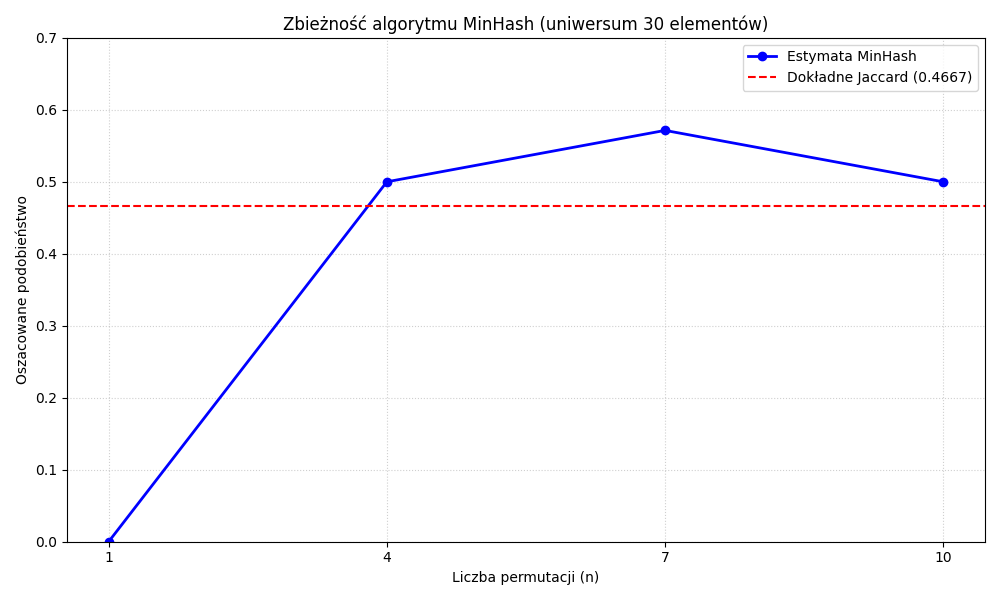
\includegraphics[width=0.8\textwidth]{MinHash.png}
    \caption{Wykres zbieżności algorytmu MinHash do wartości teoretycznej.}
    \label{fig:wykres}
\end{figure}

\subsection{Wnioski}
\begin{enumerate}
    \item \textbf{Skalowalność i metoda:} Choć w badaniu użyto jawnych permutacji dla lepszej przejrzystości, algorytm MinHash w praktyce operuje na funkcjach haszujących, co pozwala na analizę ogromnych zbiorów bez fizycznego przestawiania danych.
    \item \textbf{Analiza błędu:} Przy małej liczbie permutacji ($n=10$) błąd bezwzględny wyniósł około $0,0333$. Jest to wynik akceptowalny, biorąc pod uwagę stochastyczny charakter metody.
    \item \textbf{Zbieżność:} Eksperyment potwierdził, że udział zgodnych wierszy w macierzy sygnatur dąży do rzeczywistego podobieństwa Jaccarda wraz ze wzrostem liczby permutacji.
\end{enumerate}

\section{Zadanie 3: Wyznaczanie odległości wektorowych}

Celem zadania jest zdefiniowanie wektorów w przestrzeni wielowymiarowej, wyznaczenie odległości Euklidesowej oraz kosinusowej pomiędzy wszystkimi unikalnymi parami, a także porównanie i interpretacja obu miar.

\subsection{Definicja wektorów}
Wygenerowano 3 wektory, z których każdy składa się z 10 współrzędnych rzeczywistych z przedziału $[0, 10]$:
\begin{itemize}
    \item $v_1 = [2.0,\ 4.0,\ 1.0,\ 8.0,\ 5.0,\ 9.0,\ 3.0,\ 7.0,\ 6.0,\ 0.0]$
    \item $v_2 = [8.0,\ 1.0,\ 6.0,\ 2.0,\ 9.0,\ 0.0,\ 4.0,\ 5.0,\ 3.0,\ 7.0]$
    \item $v_3 = [1.0,\ 2.0,\ 3.0,\ 4.0,\ 5.0,\ 6.0,\ 7.0,\ 8.0,\ 9.0,\ 10.0]$
\end{itemize}

Do obliczenia odległości kosinusowej niezbędne są \textbf{normy Euklidesowe (długości)} poszczególnych wektorów, wyliczane ze wzoru $||v|| = \sqrt{\sum_{i=1}^{n} v_i^2}$:
\begin{align*}
||v_1|| &= \sqrt{2^2 + 4^2 + 1^2 + 8^2 + 5^2 + 9^2 + 3^2 + 7^2 + 6^2 + 0^2} = \sqrt{285} \approx 16,8819 \\
||v_2|| &= \sqrt{8^2 + 1^2 + 6^2 + 2^2 + 9^2 + 0^2 + 4^2 + 5^2 + 3^2 + 7^2} = \sqrt{285} \approx 16,8819 \\
||v_3|| &= \sqrt{1^2 + 2^2 + 3^2 + 4^2 + 5^2 + 6^2 + 7^2 + 8^2 + 9^2 + 10^2} = \sqrt{385} \approx 19,6214
\end{align*}

\subsection{Obliczenia pośrednie dla pary $(v_1, v_2)$}

\textbf{1. Odległość Euklidesowa $d_E(v_1, v_2)$:} \\
Wzór to suma kwadratów różnic poszczególnych współrzędnych pod pierwiastkiem.
\begin{align*}
d_E &= \sqrt{(2-8)^2 + (4-1)^2 + (1-6)^2 + (8-2)^2 + (5-9)^2 + \dots} \\
&\quad \overline{\dots + (9-0)^2 + (3-4)^2 + (7-5)^2 + (6-3)^2 + (0-7)^2} \\
d_E &= \sqrt{(-6)^2 + 3^2 + (-5)^2 + 6^2 + (-4)^2 + 9^2 + (-1)^2 + 2^2 + 3^2 + (-7)^2} \\
d_E &= \sqrt{36 + 9 + 25 + 36 + 16 + 81 + 1 + 4 + 9 + 49} \\
d_E &= \sqrt{266} \approx 16,3095
\end{align*}

\textbf{2. Odległość kosinusowa $d_C(v_1, v_2)$:} \\
Wyznaczana ze wzoru $d_C = 1 - \frac{v_1 \cdot v_2}{||v_1|| \cdot ||v_2||}$. Najpierw liczymy iloczyn skalarny:
\begin{align*}
v_1 \cdot v_2 &= (2\cdot8) + (4\cdot1) + (1\cdot6) + (8\cdot2) + (5\cdot9) + \\
&\quad + (9\cdot0) + (3\cdot4) + (7\cdot5) + (6\cdot3) + (0\cdot7) \\
v_1 \cdot v_2 &= 16 + 4 + 6 + 16 + 45 + 0 + 12 + 35 + 18 + 0 = 152
\end{align*}
Podstawiamy do głównego wzoru:
\begin{equation}
d_C = 1 - \frac{152}{\sqrt{285} \cdot \sqrt{285}} = 1 - \frac{152}{285} \approx 1 - 0,5333 = 0,4667
\end{equation}

\subsection{Obliczenia pośrednie dla pary $(v_1, v_3)$}

\textbf{1. Odległość Euklidesowa $d_E(v_1, v_3)$:}
\begin{align*}
d_E &= \sqrt{(2-1)^2 + (4-2)^2 + (1-3)^2 + (8-4)^2 + (5-5)^2 + \dots} \\
&\quad \overline{\dots + (9-6)^2 + (3-7)^2 + (7-8)^2 + (6-9)^2 + (0-10)^2} \\
d_E &= \sqrt{1^2 + 2^2 + (-2)^2 + 4^2 + 0^2 + 3^2 + (-4)^2 + (-1)^2 + (-3)^2 + (-10)^2} \\
d_E &= \sqrt{1 + 4 + 4 + 16 + 0 + 9 + 16 + 1 + 9 + 100} \\
d_E &= \sqrt{160} \approx 12,6491
\end{align*}

\textbf{2. Odległość kosinusowa $d_C(v_1, v_3)$:} \\
Iloczyn skalarny:
\begin{equation}
v_1 \cdot v_3 = 2 + 8 + 3 + 32 + 25 + 54 + 21 + 56 + 54 + 0 = 255
\end{equation}
Podstawienie do wzoru (iloczyn norm to $\sqrt{285} \cdot \sqrt{385} \approx 331,2476$):
\begin{equation}
d_C = 1 - \frac{255}{331,2476} \approx 1 - 0,7698 = 0,2302
\end{equation}

\subsection{Obliczenia pośrednie dla pary $(v_2, v_3)$}

\textbf{1. Odległość Euklidesowa $d_E(v_2, v_3)$:}
\begin{align*}
d_E &= \sqrt{(8-1)^2 + (1-2)^2 + (6-3)^2 + (2-4)^2 + (9-5)^2 + \dots} \\
&\quad \overline{\dots + (0-6)^2 + (4-7)^2 + (5-8)^2 + (3-9)^2 + (7-10)^2} \\
d_E &= \sqrt{7^2 + (-1)^2 + 3^2 + (-2)^2 + 4^2 + (-6)^2 + (-3)^2 + (-3)^2 + (-6)^2 + (-3)^2} \\
d_E &= \sqrt{49 + 1 + 9 + 4 + 16 + 36 + 9 + 9 + 36 + 9} \\
d_E &= \sqrt{178} \approx 13,3417
\end{align*}

\textbf{2. Odległość kosinusowa $d_C(v_2, v_3)$:} \\
Iloczyn skalarny:
\begin{equation}
v_2 \cdot v_3 = 8 + 2 + 18 + 8 + 45 + 0 + 28 + 40 + 27 + 70 = 246
\end{equation}
Podstawienie do wzoru:
\begin{equation}
d_C = 1 - \frac{246}{331,2476} \approx 1 - 0,7426 = 0,2574
\end{equation}

\subsection{Zestawienie i Wnioski}

\begin{table}[h!]
\centering
\caption{Porównanie odległości wektorowych dla poszczególnych par.}
\label{tab:odleglosci}
\begin{tabular}{@{}lcc@{}}
\toprule
Badana Para Wektorów & Odległość Euklidesowa ($d_E$) & Odległość Kosinusowa ($d_C$) \\ \midrule
Para $(v_1, v_2)$ & 16,3095 & \textbf{0,4667} (największa) \\
Para $(v_1, v_3)$ & \textbf{12,6491} (najmniejsza) & \textbf{0,2302} (najmniejsza) \\
Para $(v_2, v_3)$ & 13,3417 & 0,2574 \\ \bottomrule
\end{tabular}
\end{table}

\textbf{Wnioski z przeprowadzonego eksperymentu:}
\begin{enumerate}
    \item \textbf{Różnica w naturze miar:} Odległość Euklidesowa mierzy absolutną "odległość w linii prostej" w przestrzeni wielowymiarowej, silnie zależąc od modułu (wielkości) samych wektorów. Z kolei odległość kosinusowa całkowicie ignoruje długość wektorów, skupiając się wyłącznie na ich kierunku w przestrzeni (zbieżności trendów poszczególnych współrzędnych).
    \item \textbf{Interpretacja relacji między wektorami:} Wektory $v_1$ i $v_3$ są do siebie najbardziej zbliżone w świetle obu metryk. Osiągają najmniejszą odległość liniową ($d_E \approx 12,65$) oraz najmniejszą kosinusową ($d_C \approx 0,23$), co oznacza, że wykazują największe geometryczne podobieństwo.
    \item \textbf{Niezależność od długości wektora:} Ciekawym przypadkiem jest para wektorów $v_1$ i $v_2$. Pomimo faktu, że ich długości (normy $L_2$) są dokładnie takie same i wynoszą $\approx 16,88$, to w przestrzeni są one od siebie najbardziej oddalone. Ich odległość kosinusowa wyniosła aż $0,4667$, co świadczy o tym, że układ ich poszczególnych współrzędnych zmierza w zupełnie innych, wręcz przeciwstawnych w kontekście tej przestrzeni kierunkach.
\end{enumerate}

\end{document}
\end{document}